\documentclass[12pt,journal,compsoc]{IEEEtran}
\usepackage{graphicx}
\usepackage{url}
\graphicspath{ {./images/} }
% correct bad hyphenation here
\hyphenation{op-tical net-works semi-conduc-tor}

%=======================================================

\begin{document}

% Paper title
\title{CS 181W \\ Project Proposal}

% Authors
\author{Michelle~Li~\IEEEmembership{(mli6@stanford.edu)},~Thawsitt~Naing~\IEEEmembership{(thawsitt@stanford.edu)}}


% The paper headers
\markboth{CS 181W: Computers, Ethics, and Public Policy (Fall 2018)}%
{}

\maketitle

%=======================================================

\section{Introduction}

\IEEEPARstart{M}{ost} people tend to avoid thinking about ethics even though we continually make decisions about what is right or wrong in our everyday life. The goal of this project is to help people become more aware of ethical dilemmas and give them the tools to think about these situations.


\section{Project Description}
We aim to create an interactive platform (a web-app) where users will be asked to make decisions about ethically challenging situations. These will include ethical dilemmas that face normal people around the world, as well as though experiments such as the Trolley Problem. 

Users will see a summary of the situation and choose between potential actions presented in a multiple-choice style. After users have made their choice, the platform will challenge their decision and ask them to justify their decision. Users can justify their choice by ranking it on a series of moral compasses such as Utility, Rights, Common Good etc. in a way similar to SCU’s Ethics App which is discussed in Related Work section. This reflection stage is especially important as it gives the user a chance to rethink about the situation and self-discover how they make ethical decisions.

The web-app will use concise text summary, graphics, and animations to ensure an engaging experience for the users. We plan to promote the app through Stanford groups and email lists as well as internet forums such as Reddit to boost user engagement. Finally, we will use Google Analytics to measure our impact.


\section{Related Work}
MIT`s Moral Machine is ``a platform for gathering a human perspective on moral decisions made by machine intelligence, such as AVs``~\cite{mit}. Users can vote on the lesser evil in two ethical dilemmas presented side by side using graphics. It is mainly used to crowd-source public opinion on ethical dilemmas, with 30 million decisions by over 3 million visitors so far. It is different from our project in that it does not follow up on the users’ decisions. Our platform will build off of MIT’s Moral Machine by adding complexity to the scenarios, both in their presentation and the interactions with the user.

SCU`s Ethics App is ``a practical tool for thinking through tough choices``~\cite{scu}. It is a tool that lets users access their decision on five ethical perspectives, namely Utility, Rights, Justice, Common Good, and Virtue. In the end, users can choose the weight for each perspective and see how much their decision aligns with their values. We plan to use this approach in our platform as a way for users to justify and think about the decision they have made.


\newpage

\appendices

\section{}
\vspace{0.5cm}
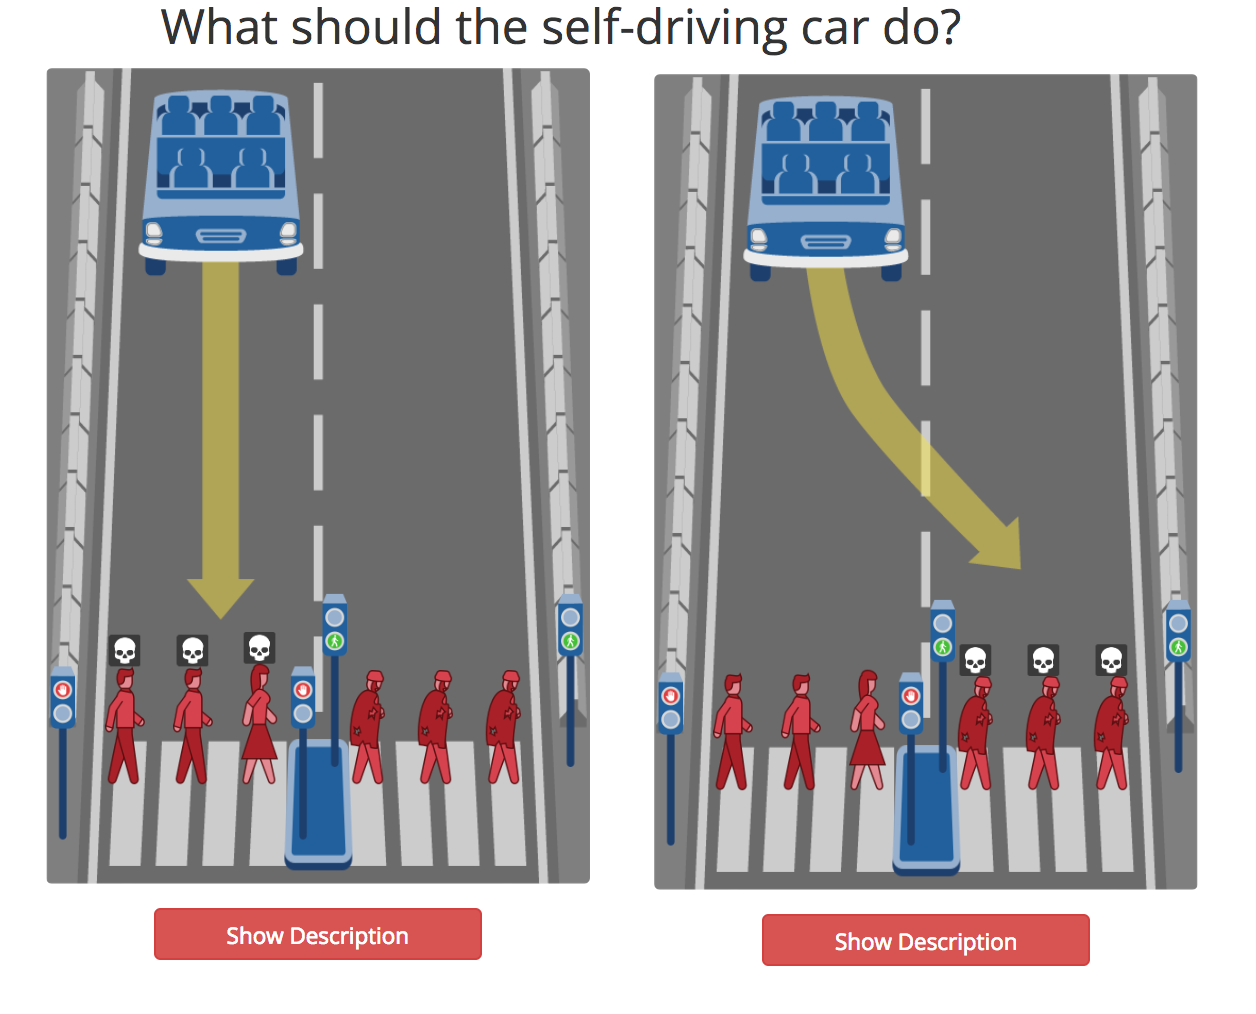
\includegraphics[width=2.5in]{images/proposal-mit.png}
\\\\ MIT's Moral Machine

\section{}
\vspace{0.5cm}
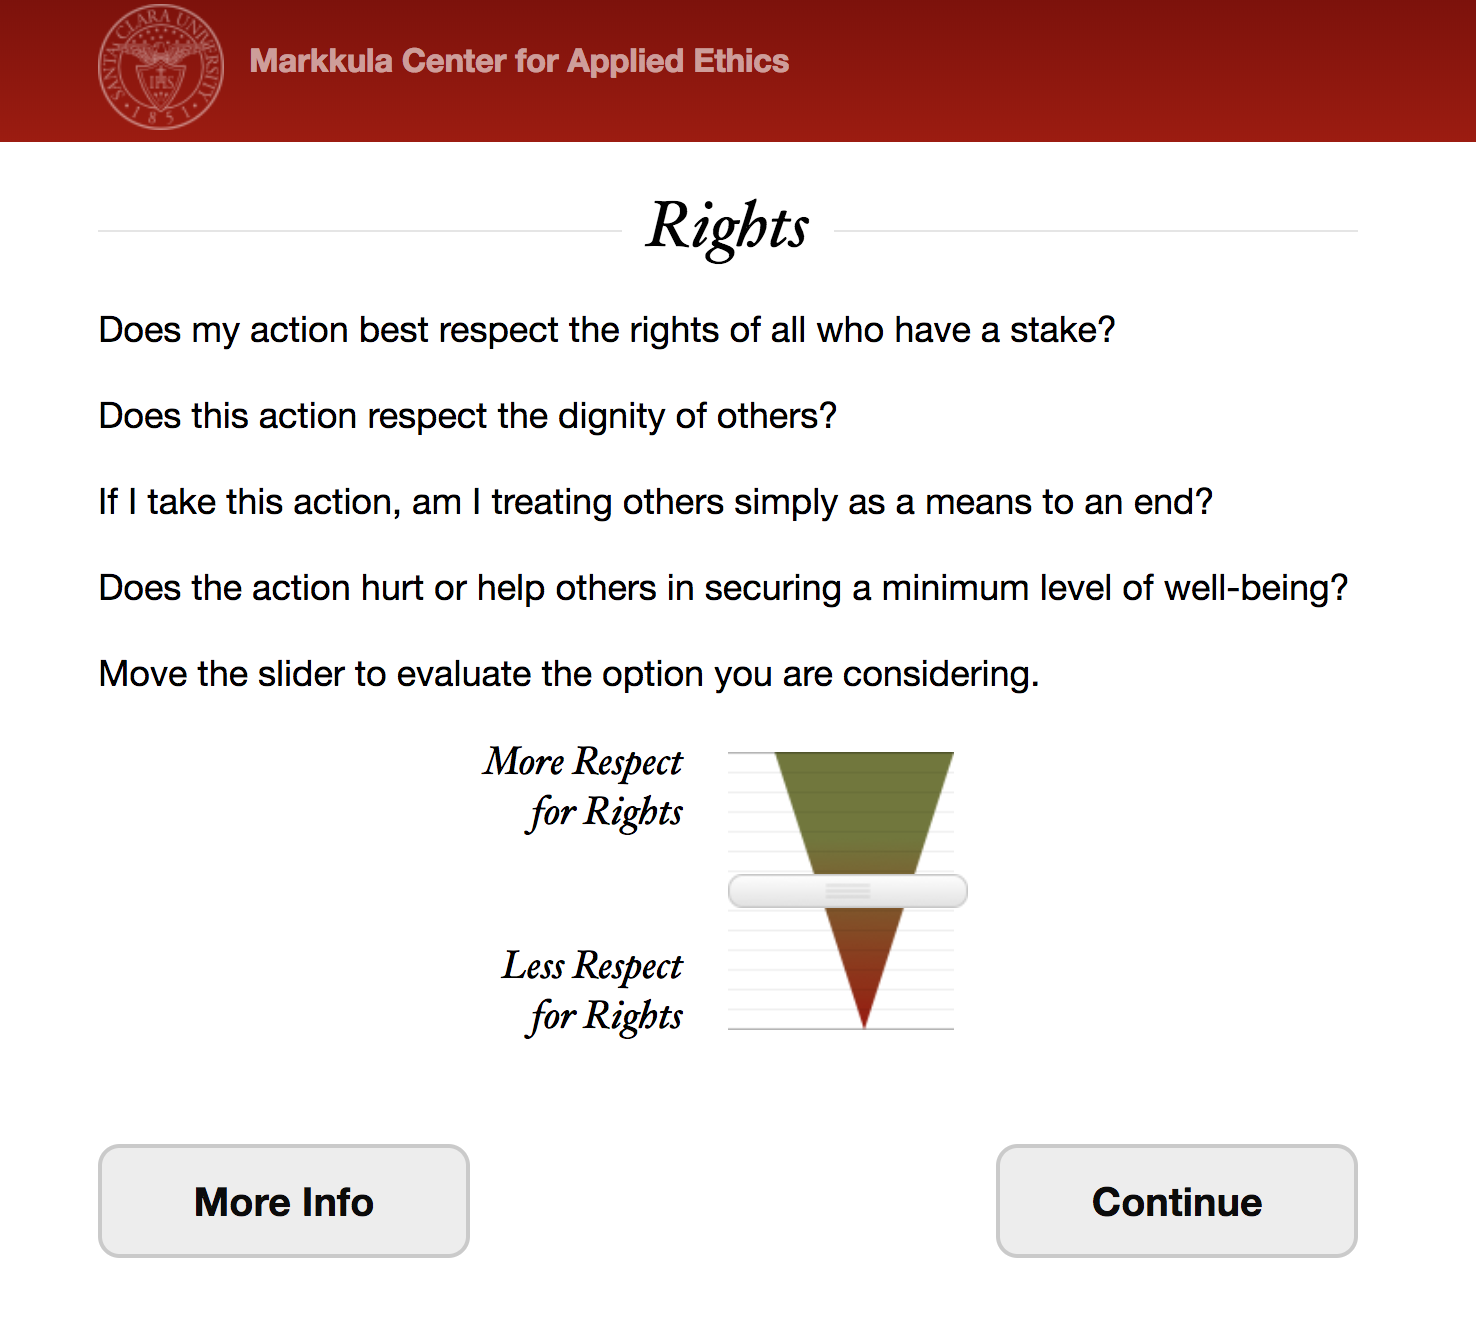
\includegraphics[width=2.5in]{images/proposal-scu.png}
\\\\ SCU's Ethics App


\ifCLASSOPTIONcaptionsoff
  \newpage
\fi

%=======================================================

\begin{thebibliography}{1}

\bibitem{mit}
MIT's Moral Machine. \\
\url{http://moralmachine.mit.edu/}

\bibitem{scu}
Santa Clara University's Ethics App\\
\url{https://www.scu.edu/ethics-app}

\end{thebibliography}


\end{document}
